\documentclass{article}
% NeurIPS 2025 style (neurips_2025.sty, in this folder) as a preprint: author names shown, no line numbers.
\usepackage[preprint,nonatbib]{neurips_2025}
\usepackage[utf8]{inputenc}
\usepackage[T1]{fontenc}
\usepackage{amsmath,amssymb}
\usepackage{booktabs}
\usepackage{array}
\usepackage{graphicx}
\usepackage{xcolor}
\usepackage{microtype}
\usepackage[numbers,sort&compress]{natbib}
\usepackage{hyperref}
\hypersetup{colorlinks=true,linkcolor=blue!50!black,citecolor=blue!50!black,urlcolor=blue!50!black}
% Generated by paper/make_assets.py from results/multiagent/; do not edit by hand.
\newcommand{\AoneEvidenceEight}{-0.11}
\newcommand{\AoneEvidenceEightCI}{[-0.14, -0.08]}
\newcommand{\AoneEvidenceEightDiff}{-0.065}
\newcommand{\AoneEvidenceFour}{-0.14}
\newcommand{\AoneEvidenceFourCI}{[-0.18, -0.09]}
\newcommand{\AoneEvidenceFourDiff}{-0.074}
\newcommand{\AoneRequestEight}{-0.17}
\newcommand{\AoneRequestEightCI}{[-0.21, -0.14]}
\newcommand{\AoneRequestEightDiff}{-0.103}
\newcommand{\AoneRequestEightP}{0.008}
\newcommand{\AoneRequestFour}{-0.18}
\newcommand{\AoneRequestFourCI}{[-0.21, -0.14]}
\newcommand{\AoneRequestFourDiff}{-0.097}
\newcommand{\AoneRequestFourP}{0.008}
\newcommand{\AoneTableEight}{-0.05}
\newcommand{\AoneTableEightCI}{[-0.09, -0.01]}
\newcommand{\AoneTableEightDiff}{-0.027}
\newcommand{\AoneTableEightP}{0.098}
\newcommand{\AoneTableFour}{-0.01}
\newcommand{\AoneTableFourCI}{[-0.06, 0.04]}
\newcommand{\AoneTableFourDiff}{-0.008}
\newcommand{\AoneTableFourP}{0.629}
\newcommand{\AsksFour}{42}
\newcommand{\AthreeDissentClassic}{0.39}
\newcommand{\AthreeDissentClassicCI}{[0.14, 0.59]}
\newcommand{\AthreeDissentLone}{-0.58}
\newcommand{\AthreeDissentLoneCI}{[-2.33, 0.13]}
\newcommand{\AthreeFactsClassic}{-0.02}
\newcommand{\AthreeFactsClassicCI}{[-0.31, 0.18]}
\newcommand{\AthreeFactsClassicP}{1.000}
\newcommand{\AthreeFactsLone}{-0.33}
\newcommand{\AthreeFactsLoneCI}{[-1.43, 0.21]}
\newcommand{\AthreeFactsLoneP}{0.860}
\newcommand{\AthreeTableClassic}{0.22}
\newcommand{\AthreeTableClassicCI}{[-0.02, 0.40]}
\newcommand{\AthreeTableClassicP}{0.292}
\newcommand{\AthreeTableLone}{0.75}
\newcommand{\AthreeTableLoneCI}{[0.50, 1.00]}
\newcommand{\AthreeTableLoneP}{0.012}
\newcommand{\AtwoRecord}{0.32}
\newcommand{\AtwoRecordCI}{[0.20, 0.44]}
\newcommand{\AtwoRecordCost}{0.006}
\newcommand{\AtwoRecordCostCI}{[-0.012, 0.026]}
\newcommand{\AtwoRecordP}{0.008}
\newcommand{\AtwoVerify}{-0.01}
\newcommand{\AtwoVerifyCI}{[-0.28, 0.19]}
\newcommand{\AtwoVerifyCost}{-0.001}
\newcommand{\AtwoVerifyCostCI}{[-0.033, 0.025]}
\newcommand{\AtwoVerifyP}{0.918}
\newcommand{\AtwoWarn}{0.03}
\newcommand{\AtwoWarnCI}{[-0.16, 0.20]}
\newcommand{\AtwoWarnCost}{0.000}
\newcommand{\AtwoWarnCostCI}{[-0.022, 0.020]}
\newcommand{\BaseHonestLoss}{0.35}
\newcommand{\BasePooledFour}{0.45}
\newcommand{\BoardBenefitFour}{0.39}
\newcommand{\BoardBenefitFourCI}{[0.37, 0.40]}
\newcommand{\CheckedFalseLiar}{13}
\newcommand{\ChecksLiar}{14}
\newcommand{\CoordBenefitFour}{0.10}
\newcommand{\CreditMinusIndividual}{0.19}
\newcommand{\CreditMinusIndividualCI}{[0.09, 0.27]}
\newcommand{\CreditMinusTeam}{0.22}
\newcommand{\CreditMinusTeamCI}{[0.14, 0.29]}
\newcommand{\CrossThreeCredit}{-0.16}
\newcommand{\CrossThreeCreditCI}{[-0.20, -0.12]}
\newcommand{\CrossThreeWarm}{-0.22}
\newcommand{\CrossThreeWarmCI}{[-0.27, -0.16]}
\newcommand{\DisclosedBase}{0.50}
\newcommand{\FollowFour}{-0.13}
\newcommand{\FollowFourCI}{[-0.16, -0.10]}
\newcommand{\GainCredit}{0.02}
\newcommand{\GainCreditCI}{[-0.03, 0.06]}
\newcommand{\GainIndividual}{-0.17}
\newcommand{\GainIndividualCI}{[-0.27, -0.07]}
\newcommand{\GainTeam}{-0.20}
\newcommand{\GainTeamCI}{[-0.26, -0.14]}
\newcommand{\PassFour}{0.12}
\newcommand{\PassFourCI}{[0.07, 0.16]}
\newcommand{\RhoBoard}{0.75}
\newcommand{\RhoBoardCI}{[0.55, 0.93]}
\newcommand{\RhoClue}{0.79}
\newcommand{\RhoClueCI}{[0.74, 0.81]}
\newcommand{\RhoForage}{0.02}
\newcommand{\RhoForageCI}{[-0.47, 0.45]}
\newcommand{\ShareHeldIndividual}{0.15}
\newcommand{\ShareHeldWarm}{0.92}
\newcommand{\SharePerHeldBase}{0.40}
\newcommand{\SharePerHeldEvidence}{0.73}
\newcommand{\SoloShareIndividual}{74}
\newcommand{\TrackACalls}{41,800}
\newcommand{\VotesAgainstBaseLone}{0.58}
\newcommand{\VotesAgainstTableLone}{0.21}
\newcommand{\WelfareCredit}{0.29}
\newcommand{\WelfareCreditCI}{[0.25, 0.32]}
\newcommand{\WelfareIndividual}{0.10}
\newcommand{\WelfareIndividualCI}{[0.03, 0.18]}
\newcommand{\WelfareTeam}{0.07}
\newcommand{\WelfareTeamCI}{[0.00, 0.13]}
\newcommand{\WelfareUntrained}{-0.001}
\newcommand{\WelfareUntrainedCI}{[-0.002, -0.000]}
\newcommand{\WelfareWarm}{0.27}
\newcommand{\WelfareWarmCI}{[0.22, 0.32]}
\newcommand{\WinBaseClassic}{0.54}
\newcommand{\WinBaseLone}{0.88}
\newcommand{\WinSolo}{1.00}
\newcommand{\WinTableLone}{0.97}
\newcommand{\WrongPerSolveIndividual}{3.8}


\title{Guards, Squads and Incentives: Keeping Large Teams of Language-Model Agents Effective and Safe}

\author{%
  Chuntao Dan \\
  \And
  Claude Opus 5.5\thanks{An AI model made by Anthropic, working as a research and coding agent in Claude Code; see the author contributions.} \\
  Anthropic \\
}

\begin{document}
\maketitle

\begin{abstract}
Teams of language-model agents trust bad information, pool less of what they know as they grow, and stop cooperating when trained with the wrong incentives. Studying teams of up to 64 Claude Haiku 5.5 agents, and reinforcement learning (RL) of a 3B open-weight model, under analysis plans frozen before the runs, we find five things. (1) \emph{Verification works as an assigned role}: guards, a quarter of the team assigned only to confirm and contest clues, recovered $\ColonyRecoverGuards$ of the damage done by an equal number of liars at 8 and 16 agents without knowing which clues were true, against $\ColonyRecoverRecord$ for an oracle record of each sender's accuracy, and beat an unprotected team at every size up to 64. (2) \emph{Splitting the team makes verification scale}: guards could check only about two in five lies, and the rest did more harm in larger teams, so their advantage shrank; squads of eight, each with its own board and guards, kept theirs, widening their lead over guards on one shared board from $\SquadsGapSixteen$ at 16 agents to $\SquadsGapSixtyFour$ at 64. (3) \emph{Larger teams are more gullible}: the share of honest answers built on a false clue rose from $\TraceContamEight$ at 8 agents to $\TraceContamThirtyTwo$ at 32, because agents treat a posted clue as settled, not because lies spread further. (4) \emph{Copies of one model do not divide labour on their own}: no agent took an offered guard role, team-reward RL created no roles, and the training reward decided whether copies kept sharing. (5) \emph{Move information; do not add work}: fixes that pass on or certify information without costing turns helped, and those that add work to every turn did not. We release the environments, plans and code that regenerate every number and figure.
\end{abstract}

\section{Introduction}

Multi-agent deployments of language models are growing, from orchestrators with parallel workers \citep{anthropic2025research} to large groups working on open-ended problems, and their failures are well documented. On hidden-profile tasks, where the right answer depends on facts that only individual members hold, groups of agents reach about 30\% accuracy where one agent with every fact reaches 81\% \citep{li2026hiddenbench}, and Anthropic's red team reports group accuracies of 17--36\% for most models \citep{anthropic2026redteam}. Agents conform \citep{weng2025conformity}, are readily misled by a single false testimony \citep{yan2026distributed}, free-ride in public goods games when they are reasoning models \citep{guzman2025corrupted}, and become opportunistic when trained with RL in social dilemmas \citep{piche2025robust}. The red team lists mechanism design, reputation and environments that shape cooperation as open problems \citep{anthropic2026redteam}.

We test fixes and how they hold up as teams grow. For each failure we build a small, fully specified environment, freeze an analysis plan before any run and add one mechanism at a time; where we can, we pair a mechanism the harness provides (an \emph{affordance}, such as a new action or observation line) with a prompt-only \emph{instruction} that gives the same advice (\S\ref{sec:methods}). Our five findings, strongest first:

\begin{enumerate}
\item \textbf{Verification works as an assigned role} (\S\ref{sec:colony}): guards, who need no ground truth, recover more of the liars' damage than an oracle track record at 8 and 16 agents, beat an unprotected team at every size from 8 to 64, and help against every kind of faulty teammate we tested.
\item \textbf{Splitting a large team makes verification scale} (\S\ref{sec:squads}): only about two in five lies fall on a clue a guard holds and, in larger teams, the other lies do more harm, so the guards' advantage shrinks; squads of eight, each with its own board and guards, keep theirs.
\item \textbf{Larger teams are more gullible, for a traceable reason} (\S\ref{sec:gullible}): replayed runs show agents in larger teams building on a posted lie more often, not lies spreading further.
\item \textbf{Copies of one model do not divide labour on their own, and the reward decides whether they cooperate} (\S\ref{sec:rl}): no agent takes up a role that is offered but not assigned, RL with a team reward does not create one, and individual reward teaches guessing instead of sharing.
\item \textbf{Move information; do not add work} (\S\ref{sec:flow}): a shared board, a coordinator that passes clues on and a public track record helped; a request board, an instruction to share first, private checks and orders to follow a coordinator did not.
\end{enumerate}

\section{Related work}

\paragraph{Information pooling in agent teams.} The hidden-profile paradigm \citep{stasser1985pooling} has been ported to LLM groups \citep{li2026hiddenbench,anthropic2026redteam}. Diagnoses stress early convergence on shared evidence \citep{li2026hiddenbench}, averaging of expert and non-expert views \citep{pappu2026experts} and loss of issue-critical facts in deliberation \citep{wan2026deliberative}; an LLM facilitator raised how much human groups shared without improving their decisions \citep{alsobay2026table}. Adaptive communication control \citep{babu2026consilience} and structured deliberation \citep{prakash2026dci} can beat unstructured discussion. Pruning messages and agents saves tokens at comparable accuracy \citep{zhang2024agentprune,wang2025agentdropout}, and across 260 configurations multi-agent architectures range from large gains to large losses against a single agent \citep{kim2025scaling}; in our tasks a message also costs its sender a turn.

\paragraph{Deception, trust and fault tolerance.} Defences learn credibility scores from past contributions \citep{ebrahimi2025credibility}, rank neighbours \citep{feng2026sentinelnet} or rectify misleading content \citep{luo2026star}. We compare a public, harness-computed signal with private verification at matched cost, and test oracle-free rules borrowed from social insects: quorum-like agreement counts \citep{seeley2010honeybee} and guards \citep{breed2004defensive}. Honest-signalling theory explains when a signal can be trusted, namely when it is costly to fake \citep{zahavi1975handicap}; our results suggest that who sees the verification, and whose job it is, matter too.

\paragraph{Training agent teams.} Multi-agent RL for LLM collaboration includes MAPoRL \citep{park2025maporl}, MAGRPO \citep{liu2026magrpo} and AT-GRPO \citep{atgrpo2025}; counterfactual credit addresses free-riding \citep{li2026ccpo,foerster2018coma}. RL-trained LLM agents become opportunistic in social dilemmas \citep{piche2025robust} and most simulated LLM societies fail to sustain a shared resource \citep{piatti2024govsim}. Grading that never penalises wrong answers rewards guessing \citep{kalai2025hallucinate}; we observe a multi-agent analogue in which agents stop sharing clues and guess, a producer-scrounger outcome \citep{barnard1981producers}.

\section{Methods}
\label{sec:methods}

\paragraph{The clue board.} $N$ agents share a board of $2N+2$ open subtasks, each worth 1, 2 or 3 points; a subtask is replaced when solved or after 30 turns. A subtask hides an integer $0 \le x < 30$ fixed by two clues ``$x \bmod p = r$'' (different primes $p$) dealt to different agents, so no agent can solve it alone. In each turn every agent takes one action: select a subtask to work on, answer the selected subtask (a wrong answer costs 0.5), share a clue, or wait. Shared clues go to a \emph{blackboard} every agent reads; in the channel comparisons they go instead to direct messages, nowhere, or to a coordinator agent that collects them and suggests subtasks. Sharing costs the sharer a turn and earns it nothing directly, so the board poses the hidden-profile problem with a price on communication.

\paragraph{Faulty teammates.} For the defences (\S\ref{sec:colony}--\S\ref{sec:squads}) each clue is dealt to two agents, so an honest holder can contradict a lie about it, and a quarter of the agents are \emph{liars}: scripted agents that, every other turn, post a false value $r$ for a clue of a subtask they are not working on. We also test \emph{mistaken} teammates, honest agents that misread 30\% of their clues; \emph{colluding} liars, who repost each other's false values and so defeat any rule that trusts a value two agents posted; and \emph{Claude liars}, Claude Haiku 5.5 agents told in a private instruction to make their teammates answer wrongly, who can act only by posting clues. In \S\ref{sec:gullible} and \S\ref{sec:flow} each clue has one holder unless stated.

\paragraph{Agents.} Team members are Claude Haiku 5.5 at the API's low effort setting. Each turn an agent receives a text observation (the open subtasks, its own clues, the board and a memory of its earlier turns) and replies with one action as JSON. Every reply is cached under its full request, so reruns are byte-identical and saved runs can be replayed with new measurements at no API cost. Rule agents written in numpy answer any subtask whose clues they know and otherwise share a clue a teammate needs for the subtask it has selected; they give a reference level and, run before each expensive study, a frozen forecast of its results (Appendix~\ref{app:sim}).

\paragraph{Mechanisms.} Each arm changes one thing (Table~\ref{tab:mech}). Where we can, an affordance is paired with an instruction that gives the same advice in one sentence of the prompt, to separate the affordance's effect from that of telling agents what to do.

\begin{table}[t]
\caption{Mechanisms tested. Kind: A, an affordance the harness provides; I, a prompt-only instruction; R, an assigned role; S, a change of team structure.}
\label{tab:mech}
\centering
\small
\begin{tabular}{@{}l>{\raggedright\arraybackslash}p{7.9cm}cc@{}}
\toprule
Mechanism & What changes & Kind & Section \\
\midrule
Blackboard & shared clues go to a board every agent reads (against no channel) & A & \ref{sec:flow} \\
Follow the coordinator & agents are told the coordinator sees every shared clue and its suggestion is usually best & I & \ref{sec:flow} \\
Coordinator passes clues & with each suggested subtask, the coordinator passes on the clues it has collected for it & A & \ref{sec:flow} \\
Request board & a new action asks teammates for the clues of the agent's selected subtask & A & \ref{sec:flow} \\
Share first & ``post every clue you hold for an open subtask before working on your own'' & I & \ref{sec:flow} \\
Clue table & for each open subtask, the board lists the clues the team has posted so far & A & \ref{sec:flow} \\
Track record & beside each clue, how many of its sender's earlier clues proved true (needs the truth) & A & \ref{sec:flow} \\
Check action & spend a turn to learn privately whether a posted clue is true & A & \ref{sec:flow} \\
Warning & ``a teammate may share false clues; cross-check before relying on one'' & I & \ref{sec:flow} \\
Agreement counts & the board counts the agents that posted each value and marks it confirmed or contested & A & \ref{sec:colony} \\
Instruction only & agents are told to confirm or contest values; no counts shown & I & \ref{sec:colony} \\
Guards & a quarter of the team (as many as the liars) is told to post, confirm and contest clues, never to solve & R & \ref{sec:colony} \\
Volunteer offer & the guard role and its rationale are offered to every agent, with no assignment & I & \ref{sec:rl} \\
Squads & the team splits into squads of eight, each with its own board, subtasks and two guards & S & \ref{sec:squads} \\
Failure flags & after a wrong answer, the board flags the posted values it agreed with & A & \ref{sec:squads} \\
Guard copies & one of each clue's two copies is dealt to a guard & A & \ref{sec:squads} \\
Vote fixes & hidden-profile vote: a fact table (A), a facts-only first round (A), a speak-up instruction (I) & A, I & \ref{sec:vote} \\
\bottomrule
\end{tabular}
\end{table}

\paragraph{Training.} We trained Qwen2.5-3B-Instruct on the clue board (four agents, blackboard) as teams of copies of one model sharing a LoRA adapter. A supervised warm start imitated the rule agent's moves (about $\WarmTurns$ turns in teams of one, two and four). RL then used group-relative policy gradients: each step played 8 boards 4 times each; each agent slot's return was compared with that slot's mean over the four plays, and each update used a random quarter of the turns with a nonzero advantage, with a KL penalty toward the warm start. The learning rate was steered to a target per-step policy change (a KL of 0.003, measured on re-scored replies), steps that moved the policy more than four times the target were undone, and runs halted on persistent invalid replies or on large drift from the warm start. Rewards were \emph{individual} (an agent's own points less its penalties), \emph{team} (the mean of the team's individual rewards), \emph{credit} (the solver keeps half of a subtask's value and the rest goes to the agents whose shared clues it used) and \emph{individual + penalty} (individual reward with a training-only penalty: a wrong answer costs 3 instead of 0.5). Trained models were scored on 15 held-out boards by welfare, whatever their training reward.

\paragraph{Measures.} \emph{Welfare} is points earned, net of penalties, per agent-turn. The \emph{pooled share} divides welfare by what the same board would yield if every clue were known to all, so 1 is the information ceiling; with liars present we report the honest agents' pooled share. The \emph{honest loss} is the honest agents' welfare without liars minus with them, on the same seed and arm, and \emph{loss recovered} is $1 -$ (arm's mean honest loss / baseline's). \emph{Gap closed} is the mean paired difference (arm minus baseline) divided by the ceiling minus the baseline, so 1 closes the gap and a negative value widens it. An answer is \emph{built on a false clue} if it agrees with a false value posted before it. \emph{Specialization} is the variance across honest agents of how often each shares, relative to binomial noise, minus the same index with turns shuffled between agents (0: no more than chance).

\paragraph{Design and statistics.} Each study's analysis plan (arms, seeds, primary tests and correction family) was frozen, hashed and committed before its runs (Appendix~\ref{app:repro}); the larger-team stages of \S\ref{sec:colony} and \S\ref{sec:squads} were declared deviations, each with its own frozen plan. Arms are paired on board seed and compared through their paired differences, as \citet{miller2024errorbars} recommends for evaluations, with 5 to 10 seeds per arm (8 for the defences). Tests are paired sign-flip tests over seeds, or over training runs when RL designs are compared (exact, or with at least 10{,}000 random sign flips when there are too many units to enumerate), one-sided where the plan fixed a direction; team sizes are compared by exact permutation tests. Holm correction applies within each plan's primary family. A trend over team size is the mean of each seed's least-squares slope against $\log_2 N$ (change per doubling of the team), tested with a two-sided sign-flip test over seeds; trends are descriptive. With three sizes evenly spaced in $\log_2 N$ the slope depends only on the smallest and largest, so we also report the change between neighbouring sizes. In the text, brackets give 95\% bootstrap intervals over the pairing units. In the figures, points and bars are means, error bars are one standard error of the mean (SEM) over seeds or boards (the bootstrap standard error for ratio measures), and an asterisk marks $p < 0.05$ in an uncorrected two-sided test against the stated reference. Because several stages were added after earlier results, we treat all findings as exploratory.

\section{Results}

\subsection{Verification works as an assigned role}
\label{sec:colony}

Here one agent in four lies and the harness does not know which clues are true. At 8 and 16 agents (8 seeds; plan \texttt{\ColonyPlanHash}; API cost \$\ColonyCost) we compared the \emph{plain board} (no defence), agreement counts (the \emph{counting board}), the same advice as an instruction, agreement counts with guards, and an oracle track record of each sender (Figure~\ref{fig:guards}).

\begin{figure}[t]
\centering
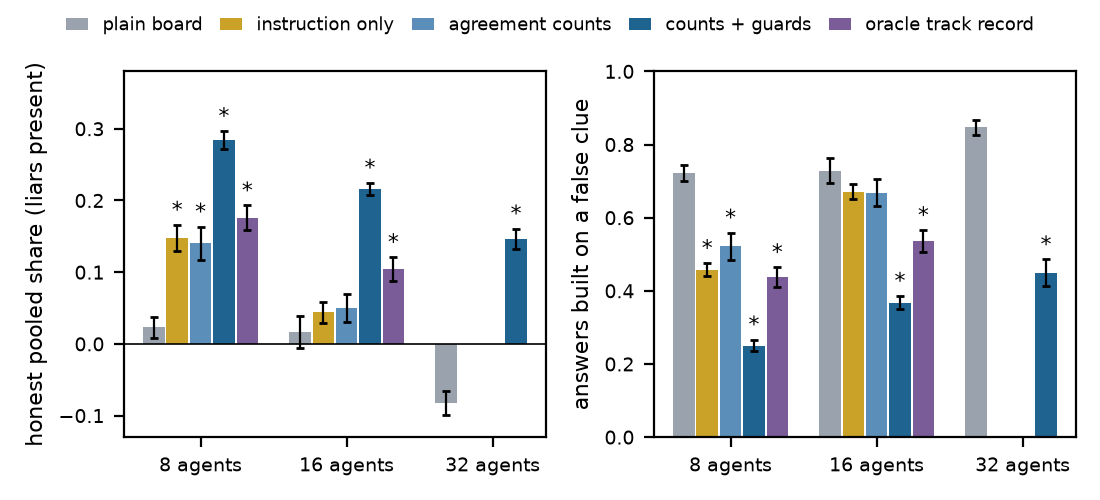
\includegraphics[width=0.94\linewidth]{figures/guards.png}
\caption{Defences against liars (a quarter of the agents), 8 seeds per bar; at 32 agents only the plain board and guards ran. Left: the honest agents' pooled share. Right: the share of honest answers built on a false clue. Mean $\pm$ SEM; * $p < 0.05$ against the plain board, two-sided exact sign-flip test paired on seed, uncorrected.}
\label{fig:guards}
\end{figure}

\textbf{Guards worked.} They beat the counting board by $\ColonyGuards$ $\ColonyGuardsCI$ in the honest agents' pooled share (Holm $p \ColonyGuardsHolm$) and recovered $\ColonyRecoverGuards$ of the liars' damage over the two sizes, against $\ColonyRecoverRecord$ for the oracle record. They did so by making checking a few agents' only job: with guards, each lie drew $\ColonyGuardContest$ contests from honest agents (counting board $\ColonyBoardContest$, plain board $\ColonyPlainContest$), and the share of honest answers built on a lie fell to $\ColonyGuardContam$ (counting board $\ColonyBoardContam$, plain board $\ColonyPlainContam$). \textbf{The display added nothing to the advice.} The counting board beat the plain board ($\ColonyBoard$ $\ColonyBoardCI$) but did no better than the one-sentence instruction (difference $\ColonyVsConfirm$), and some honest agents reposted a lie to ``confirm'' it.

\textbf{Guards held at every size and against every fault we tested.} Guards beat the plain board by $\GuardsByEight$, $\GuardsBySixteen$, $\GuardsByThirtyTwo$ and $\GuardsBySixtyFour$ at 8, 16, 32 and 64 agents, in $\GuardsByPositive$ of $\GuardsBySeeds$ seeds at each size (one-sided exact $p = \GuardsByP$ each). At 32 agents they also helped against mistaken teammates ($\GuardsThirtyTwoMistaken$ $\GuardsThirtyTwoMistakenCI$, $p = \GuardsThirtyTwoMistakenP$) and against colluding liars ($\GuardsThirtyTwoCollude$ $\GuardsThirtyTwoColludeCI$, $p = \GuardsThirtyTwoColludeP$): a guard contests a wrong value of a clue it holds however many agents posted it. At 16 agents (plan \texttt{\StagePlanHash}) we replaced the scripted liars with Claude liars. Guards still beat the plain board ($\StageAdaptive$ $\StageAdaptiveCI$, Holm $p = \StageAdaptiveHolm$) and recovered $\StageRecoverAdaptive$ of the Claude liars' damage ($\StageRecoverScripted$ for scripted liars in the same run). The Claude liars lied less often than scripted ones (a false post in $\StageLiarRate$ of their turns, against 0.5), did as much damage per lie, and did not avoid clues a guard held.

\textbf{The cost.} On boards without liars (\emph{clean} boards), guards cost $\GuardsCleanEight$, $\GuardsCleanSixteen$ and $\GuardsCleanThirtyTwo$ pooled share at 8, 16 and 32 agents: a quarter of the team checks instead of solving.

\subsection{Splitting a large team makes verification scale}
\label{sec:squads}

\begin{figure}[t]
\centering
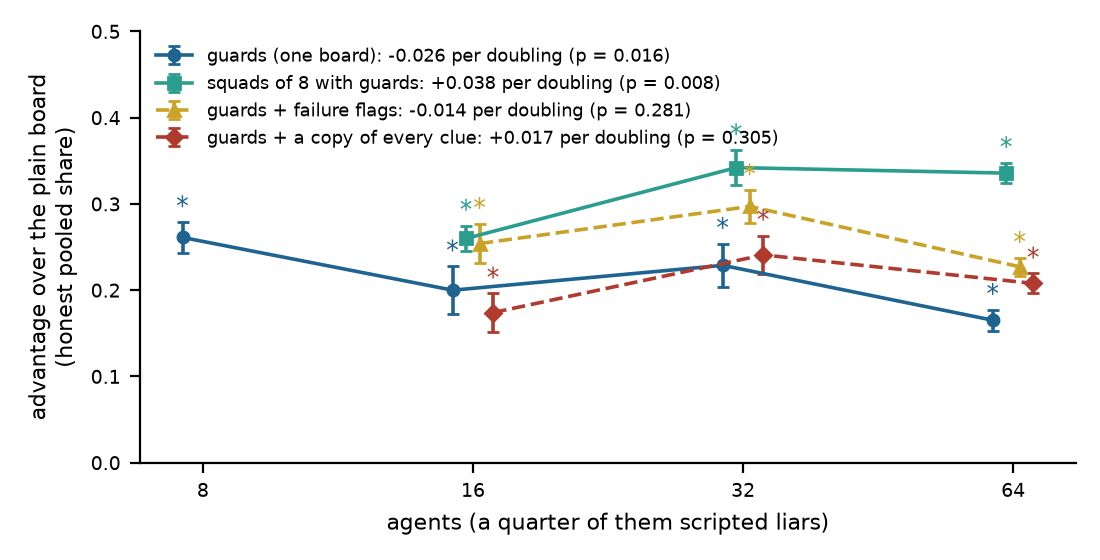
\includegraphics[width=0.94\linewidth]{figures/guards_scale.png}
\caption{Advantage over the plain board in the honest agents' pooled share against team size, a quarter of the agents scripted liars, 8 seeds per point (the three design changes ran at 16, 32 and 64 agents). Mean $\pm$ SEM; * $p < 0.05$, two-sided exact sign-flip test against 0, paired on seed, uncorrected. The legend gives each design's trend: the mean of each seed's slope over $\log_2$ of the team size, per doubling, with its two-sided exact sign-flip $p$ (descriptive; with three sizes evenly spaced on this scale, as for the design changes, the slope depends only on the smallest and largest). Guards on one board lose ground as teams grow; squads of eight, each with its own board and guards, rise from 16 to 32 agents and hold that level at 64.}
\label{fig:scale}
\end{figure}

From 8 to 64 agents the guards' advantage over the plain board changed by $\GuardsTrendSixtyFour$ per doubling of the team (two-sided $p = \GuardsTrendSixtyFourP$; descriptive). Replaying every guard board from the response cache showed that the guards themselves did not weaken. At every size they contested $\DiagContestMin$--$\DiagContestMax$\% of the lies on clues they held, with a median delay of $\DiagLagMin$--$\DiagLagMax$ turns, and each such lie led to only $\DiagUsesGuardedMin$--$\DiagUsesGuardedMax$ wrong answers. The limit is coverage: with two holders per clue, only $\DiagHeldMin$--$\DiagHeldMax$\% of lies fell on a clue a guard held. Lies on the other clues caused $\DiagUnguardedMin$--$\DiagUnguardedMax$\% of all answers built on a lie, and each caused more wrong answers in larger teams ($\DiagUsesUnguardedEight$ at 8 agents, $\DiagUsesUnguarded$ at 64). On the plain board, too, each lie did more harm in larger teams ($\PlainUsesPerLieEight$ wrong answers at 8 agents, $\PlainUsesPerLieSixtyFour$ at 64), but there the liars already took nearly everything the honest agents earned (honest pooled share $\GuardsEightPlainLiar$ with liars against $\GuardsEightPlainClean$ on clean boards at 8 agents; $\GuardsThirtyTwoPlainLiar$ against $\GuardsThirtyTwoPlainClean$ at 32), so its loss had little room to grow. The guarded board's loss did grow, and the share of the damage guards recovered fell from $\GuardsRecoverEight$ at 8 agents to $\GuardsRecoverSixteen$ at 16 and $\GuardsRecoverThirtyTwo$ at 32.

We then tested three design changes against guards on one shared board at 16 and 64 agents (plan and numpy forecast frozen first, \texttt{\FourPlanHash}; \$\FourCost). All three beat them at 64 agents, each in $\FourPositive$ of $\FourSeeds$ seeds (one-sided, Holm $p = \FourSquadsHolm$ each), and on raw welfare too (Figure~\ref{fig:scale}). \emph{Squads} won by $\FourSquads$ $\FourSquadsCI$ at 64 agents, and their advantage over the plain board rose from $\FourAdvSquadsSixteen$ at 16 agents to $\FourAdvSquadsSixtyFour$ at 64, in $\FourSquadsSlopeRising$ of 8 seeds ($\FourSquadsSlope$ per doubling, two-sided exact $p = \FourSquadsSlopeP$; descriptive), while that of guards on one board fell (the squads' change minus the guards': $\FourSquadsDid$ $\FourSquadsDidCI$, $p = \FourSquadsDidP$); a 64-agent team of squads kept $\FourSquadsLevel$ honest pooled share, near the 8-agent guard board's $\FourGuardsEightLevel$, with prompts of \FourSquadsTokens{} tokens per turn instead of \FourBoardTokens{} on one board. \emph{Failure flags} make public what the environment already tells the agent whose answer failed; they added $\FourFlags$ $\FourFlagsCI$ at 64 agents and $\FourFlagsSixteen$ at 16, at no cost on clean boards ($\FourFlagsClean$), though $\FourFlagsOnTrue$ of flags fell on true values. \emph{Guard copies} helped only at 64 agents ($\FourCopies$ $\FourCopiesCI$): at 16 they cost $\FourCopiesClean$ pooled share on clean boards, and at 64 agents, guards holding every clue contested $\FourCopiesContest$ of the lies on their clues, against $\FourGuardsContest$ for ordinary guards. Two sizes cannot show a trend's shape, so we added 32 agents for all three designs (a declared deviation; plan and forecast frozen first, \texttt{\FourBPlanHash}; \$\FourBCost). At 32 agents squads and failure flags again beat guards on one board ($\FourBSquads$ $\FourBSquadsCI$ and $\FourBFlags$ $\FourBFlagsCI$, Holm $p = \FourBSquadsHolm$ each, each in $\FourBPositive$ of $\FourSeeds$ seeds), while guard copies drew level ($\FourBCopies$ $\FourBCopiesCI$, Holm $p = \FourBCopiesHolm$), between their loss at 16 agents and their win at 64. The squads' advantage over the plain board rose from 16 to 32 agents ($\SquadsStepUp$, $p = \SquadsStepUpP$, up in $\SquadsStepUpSeeds$ of 8 seeds) and then held ($\FourAdvSquadsThirtyTwo$ at 32, $\FourAdvSquadsSixtyFour$ at 64; change $\SquadsStepFlat$, $p = \SquadsStepFlatP$), while the advantage of guards on one board fell to $\FourAdvGuardsSixtyFour$ at 64, so the squads' lead over them widened from $\SquadsGapSixteen$ at 16 agents to $\SquadsGapThirtyTwo$ at 32 and $\SquadsGapSixtyFour$ at 64 (descriptive). Verification has a capacity limit, and small groups with their own checkers scale where one global board does not. Squads shared no subtasks, so their gain holds for tasks that split cleanly and is likely an upper bound for tasks that do not.

\subsection{Larger teams are more gullible}
\label{sec:gullible}

Without a defence, the same share of liars does more damage in a larger team. With one holder per clue and a quarter of the agents liars (5 seeds), the honest loss was higher at 16 and 32 agents ($\ScaleLossSixteen$ and $\ScaleLossThirtyTwo$) than at 8 ($\ScaleLossEight$); with two holders per clue, liars pushed the plain board's honest pooled share below zero at 32 and 64 agents ($\GuardsThirtyTwoPlainLiar$ and $\GuardsSixtyFourPlainLiar$), and at 64 agents $\GuardsSixtyFourContamPlain$ of honest answers were built on a lie. A numpy rule-agent forecast frozen before the runs had predicted that the loss would fall.

\begin{figure}[t]
\centering
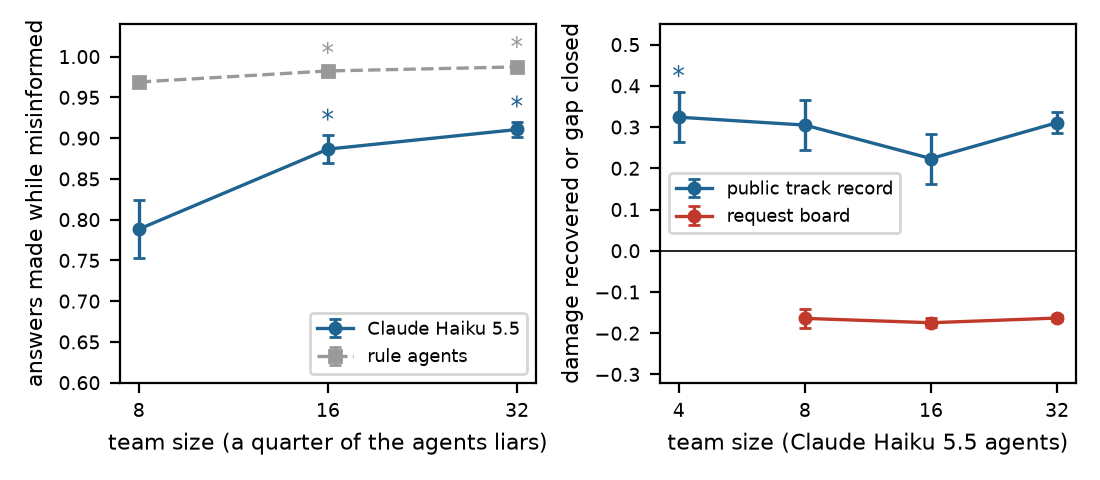
\includegraphics[width=0.94\linewidth]{figures/trust_scale.png}
\caption{Left: share of honest answers built on a false clue, one holder per clue and a quarter of the agents liars, for Claude Haiku 5.5 (5 seeds) and rule agents (20 seeds); mean $\pm$ SEM; * $p < 0.05$, exact permutation test against 8 agents. Right: share of the liars' damage recovered by the public track record and share of the pooling gap closed by the request board, against team size (10 seeds at 4 agents, 5 at larger sizes); mean $\pm$ bootstrap SE; * $p < 0.05$, two-sided exact sign-flip test against 0 (with five seeds the exact two-sided $p$ cannot fall below 0.0625).}
\label{fig:trust}
\end{figure}

We replayed the one-holder runs from the response cache with a turn-by-turn tracer (plan \texttt{\TracePlanHash}; no API calls) and split the honest loss into additive terms that sum to it exactly. Lies were no more visible in larger teams (a similar share of open subtasks showed a false value), and honest agents almost never reposted a liar's value (at most $\TraceRelayMax$\% of liar posts). What grew was how often agents built on a lie: the share of honest answers built on a false clue rose from $\TraceContamEight$ at 8 agents to $\TraceContamThirtyTwo$ at 32 (Figure~\ref{fig:trust}, left), such answers were wrong \TraceWrongContam\% of the time, and losses on subtasks a lie touched accounted for $\TraceShareAC$ of the rise in honest loss. When a liar was first to post a clue, no honest agent posted its true value afterwards in \TraceSuppress\% of cases: agents treat a posted clue as settled, whoever posted it. This is the failure guards repair, by contesting the settled clue. Two fixes first tested at four agents (\S\ref{sec:flow}) kept their effect as teams grew (Figure~\ref{fig:trust}, right): with a quarter of the agents liars, the public track record recovered $\ScaleRecordEight$, $\ScaleRecordSixteen$ and $\ScaleRecordThirtyTwo$ of the loss at 8, 16 and 32 agents, and the request board hurt pooling about as much at every size.

\subsection{Copies of one model do not divide labour on their own}
\label{sec:rl}

\textbf{Prompting.} Offered the guard role and its rationale but no assignment (16 agents), no honest agent acted as a guard on any of $\VolunteerBoards$ boards: the team did no better than the counting board alone ($\StageVolunteer$ $\StageVolunteerCI$, Holm $p = \StageVolunteerHolm$) and scored $\StageVolunteerVsGuards$ relative to assigned guards.

\textbf{Training.} Imitation did most of the teaching: the warm start raised welfare from $\WelfareUntrained$ (untrained) to $\WelfareWarm$ $\WelfareWarmCI$ (Figure~\ref{fig:rl}). The reward decided what RL added. Under individual reward the model stopped sharing ($\ShareHeldWarm$ to $\ShareHeldIndividual$ shares per held clue) and solved by guessing ($\SoloShareIndividual$\% of solves): with a wrong answer costing 0.5, guessing in turn through three remaining candidates for a 3-point subtask earns about 1.25 points per turn, while sharing earns the sharer nothing. The team-reward run collapsed mid-training and was halted; credit reward kept agents sharing and beat individual reward by $\CreditMinusIndividual$ $\CreditMinusIndividualCI$. The training-only penalty on wrong answers suppressed guessing in every run ($\GuessesPenMin$--$\GuessesPenMax$ guesses per board against $\GuessesIndMin$--$\GuessesIndMax$). We had also claimed that it kept agents sharing, but a pre-registered replication (four runs without the penalty, five with it) found that effect seed-dependent ($\SixteenShare$ shares per held clue, exact $p = \SixteenShareP$, Holm $\SixteenShareHolm$; the selfish drift appeared in only $\SixteenDrift$ of the four runs without the penalty), and we withdrew the claim.

\begin{figure}[t]
\centering
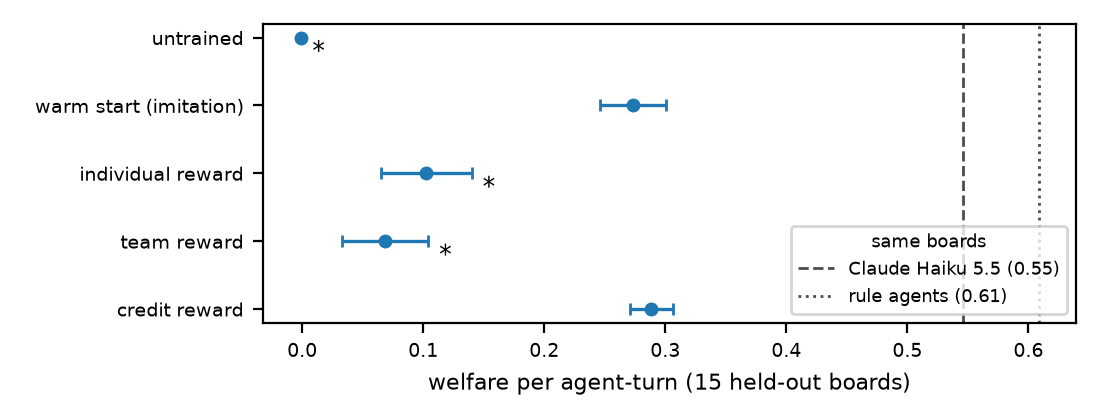
\includegraphics[width=0.94\linewidth]{figures/rl_main.png}
\caption{Welfare per agent-turn of trained four-agent teams of Qwen2.5-3B-Instruct on 15 held-out boards: the untrained model, the warm start and one training run per reward, with Claude Haiku 5.5 and rule agents on the same boards for reference. Mean $\pm$ SEM over boards; * $p < 0.05$ against the warm start, two-sided exact sign-flip test paired on board, uncorrected.}
\label{fig:rl}
\end{figure}

\textbf{Roles did not emerge.} Five runs of 30 steps with team reward on the counting board and no role instruction (plan \texttt{\PartBPlanHash}) all ran without a halt, but the trained teams' specialization averaged only $\PartBSpec$ (exact $p = \PartBSpecP$, not significant), below the warm start's $\PartBWarmSpec$ before any RL; the most specialized trained run reached $\PartBMaxSpec$. Of the five runs, $\PartBCollapsed$ collapsed to every agent posting and none solving: under team reward a post is never penalized and an answer can be. Training on mixed four- and eight-agent teams (8 runs of 60 steps; plan \texttt{\SeventeenPlanHash}) raised welfare at four agents from $\SeventeenWarmFour$ to $\SeventeenTrainedFour$ in $\SeventeenPositive$ of 8 runs (exact $p = \SeventeenGainP$; Holm $\SeventeenGainHolm$, not significant after correction), but not at 32 agents ($\SeventeenTrainedThirtyTwo$ against $\SeventeenWarmThirtyTwo$ for the warm start; Claude Haiku reaches $\SeventeenHaikuThirtyTwo$); trained teams did lose less to liars at 32 agents (reduction in honest loss $\SeventeenLiar$ $\SeventeenLiarCI$, $p = \SeventeenLiarP$, a secondary test). Training at small sizes did not teach what large teams need.

\textbf{A training lesson.} Of those 8 runs, $\SeventeenHalted$ halted early, $\SeventeenKLHalts$ of them on the drift rule: in $\SeventeenFlatHalts$ the logged KL to the warm start jumped in one step while the measured policy change and behaviour stayed flat, and in $\SeventeenBadHalts$ a single update went wrong and was undone. The per-token estimate $e^{d} - d - 1$ ($d$: the reference's log-probability of a sampled token minus the policy's) grows exponentially when the policy makes a token far less likely than the reference does, so one token can dominate the logged mean and, through the loss, an update. Capping each token's term and requiring two consecutive steps over the threshold removed the false halts.

\subsection{Move information; do not add work}
\label{sec:flow}

\begin{figure}[t]
\centering
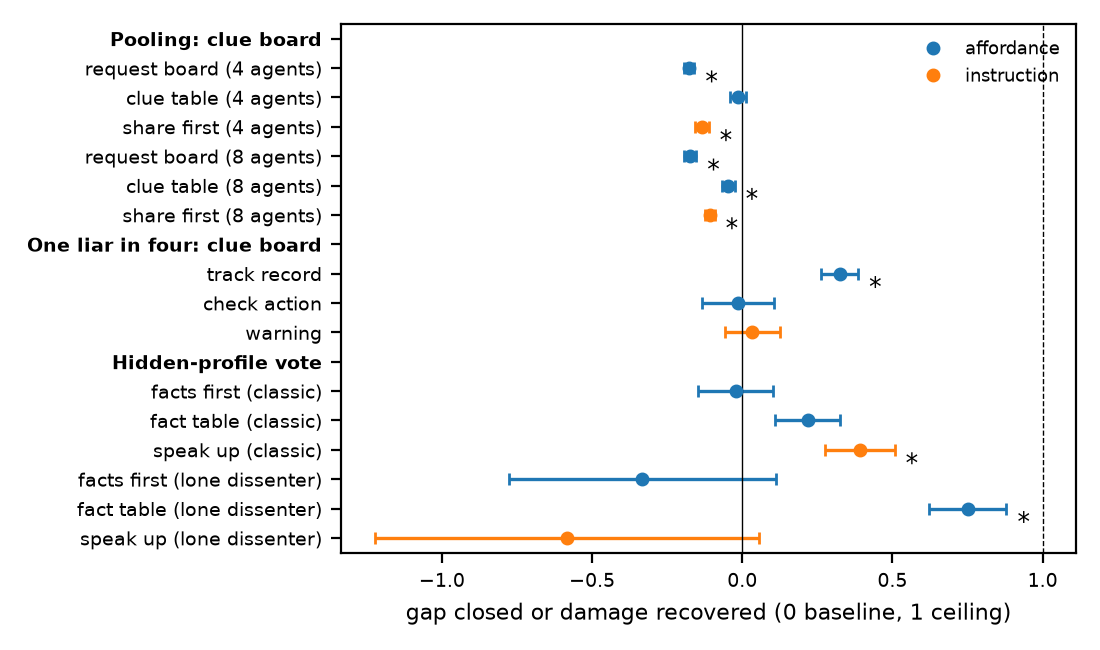
\includegraphics[width=0.94\linewidth]{figures/fixes.png}
\caption{Each fix at four agents (eight where marked; Table~\ref{tab:mech}): share of the gap to the ceiling closed (pooling, vote) or of the liar's damage recovered (one liar), where 0 is the baseline and 1 the ceiling (dashed). In the vote, \emph{facts first} allows only facts in round one, \emph{fact table} lists the facts posted and \emph{speak up} asks members to share what others seem to lack; in the \emph{lone dissenter} variant one member also holds a decisive fact. Blue: affordances; orange: prompt-only instructions. Mean $\pm$ bootstrap SE over the pairing units (10 seeds on the clue board, 100 episodes in the vote); * $p < 0.05$, two-sided sign-flip test of the paired difference against the baseline (exact over seeds; 10{,}000 random sign flips over episodes), uncorrected (the text gives the plan's Holm-corrected tests).}
\label{fig:fixes}
\end{figure}

\textbf{Channels and coordinators.} A blackboard added $\BoardBenefitFour$ $\BoardBenefitFourCI$ welfare per agent-turn over no channel at four agents. A coordinator that collects clues and suggests subtasks added only $\CoordBenefitFour$. Against that coordinator, telling agents to follow its suggestions hurt ($\FollowFour$ $\FollowFourCI$), as they selected subtasks for which they held no clue and waited for clues it never passed on, while having it pass on the clues it had collected helped ($\PassFour$ $\PassFourCI$). A coordinator helps by moving information, not by giving orders.

\textbf{Communication has a price.} The baseline team earned a pooled share of $\BasePooledFour$ at four agents. Agents asked through the request board in $\AskShareFour$ of their turns, yet sharing did not rise and the gap to the ceiling widened (gap closed $\AoneRequestFour$ $\AoneRequestFourCI$ at four agents, Holm $p = \AoneRequestFourP$; about the same at 8, 16 and 32: $\ScaleRequestEight$, $\ScaleRequestSixteen$, $\ScaleRequestThirtyTwo$). A clue table did not help ($\AoneTableFour$ $\AoneTableFourCI$ at four agents, $\AoneTableEight$ at eight, Holm $p = \AoneTableEightP$). An instruction to post every held clue first raised sharing from $\SharePerHeldBase$ to $\SharePerHeldEvidence$ shares per held clue but widened the gap ($\AoneEvidenceFour$ $\AoneEvidenceFourCI$): each post costs a turn that could have gone to solving (Figure~\ref{fig:fixes}).

\textbf{Public reputation, not private verification.} With one liar among four agents, the track record recovered $\AtwoRecord$ $\AtwoRecordCI$ of the honest agents' loss (Holm $p = \AtwoRecordP$), at no cost without a liar ($\AtwoRecordCost$). The check action caught lies but recovered none of the loss ($\AtwoVerify$ $\AtwoVerifyCI$): a check cost a turn and informed only the checker. A warning did nothing ($\AtwoWarn$). A $2 \times 2$ design crossing public or private with free or costly verification (10 seeds) found that making it public raised the share of loss recovered by $\TrustPublicity$ $\TrustPublicityCI$ and making it free by $\TrustCost$ $\TrustCostCI$: both matter, about equally. Unlike guards, the record needs the harness to know the truth.

\section{Discussion}

\paragraph{Where to put the work.} The mechanisms that helped made information easier to move or to trust at no cost in turns (a shared board, a public record) or gave checking to agents whose job it was (guards); those that failed added work to every agent's turn (asking, checking, sharing first), demanded obedience, or only displayed what agents could infer for themselves (agreement counts, no better than an instruction, and a clue table). For harnesses this suggests: put verification in the environment or in a role, not in every agent's turn; and keep each verifier's span small enough to cover what it must check, by splitting large teams into squads rather than growing one global board.

\paragraph{From assigned to trained roles.} Assigned roles worked; offered roles were not taken; and team reward neither created roles nor kept every run productive. Roles will likely have to be trained, with a reward that pays an agent when others use its contribution, as credit reward did for sharing.

\paragraph{Future directions.} Four experiments follow directly. (i) \emph{Train roles rather than reward teams}: a role-conditioned or credit-style reward that pays a guard when its contest prevents a wrong answer, evaluated against the warm start. (ii) \emph{Squads on coupled tasks}: subtasks whose clues span squads, with bridge agents that carry clues between them, to measure how much of the squads' gain survives when a task does not split cleanly. (iii) \emph{Stronger adversaries}: Claude liars in 64-agent teams, liars that target the clues no guard holds, and free-text persuasion, against squads and failure flags. (iv) \emph{Correlated errors and real tasks}: teams in which every copy shares a blind spot, guards drawn from a different model, and verification on coding or research tasks where a check costs more than a turn. We would start with (ii), the cheapest test of the squads result, and treat (i) as the main project. For all four, a simulator that captured what our rule-agent forecasts missed, such as building on a posted lie, could rank designs before any API spend.

\paragraph{Limitations.} The tasks are small and synthetic; the Claude teams use one model (Haiku 5.5) and mostly scripted liars; Claude liars could act only through clue posts; correlated errors shared by every copy of a model and compromised agents remain untested. Board arms have 5--10 seeds and RL designs one to eight training runs, which the failed replication (\S\ref{sec:rl}) shows is too few to rank similar designs; RL used a 3B model trained at four and eight agents only. The trust fixes have not been tested on a dedicated misinformation benchmark such as ForesightSafety-TIDE \citep{yan2026distributed}.

\paragraph{Broader impact.} The mechanisms studied are defensive or improve cooperation; the RL results show how easily a plausible incentive teaches agents to abandon cooperation, which matters for anyone training groups of models.

\section*{Author contributions}
Chuntao Dan directed the project: chose the questions and the order of the studies, made the design decisions recorded in the specifications, ran the GPU training and reviewed every result. Claude Opus 5.5, working as an agent in Claude Code under that direction, wrote the specifications, analysis plans, environments and analysis code, ran the API experiments and replays, analysed the results and drafted the paper. Chuntao Dan takes responsibility for the content.

\bibliographystyle{plainnat}
\bibliography{references}

\appendix
\section{Reproducibility}
\label{app:repro}
Code, environments and notebooks: \url{https://github.com/Positron00/explRL}; a highlights page redraws the main figures from a compact extract of the saved runs (\url{https://positron00.github.io/explRL/highlights.html}). Analysis plans were frozen and committed before their runs; each hash is the first 12 hexadecimal digits of the SHA-256 of the plan's canonical JSON (fixes: \texttt{FIX\_PLAN}, hash \texttt{79abfb531cdd}; RL: \texttt{RL\_PLAN} v2, hash \texttt{4d1ea0078a6e}; second RL round: \texttt{RL13\_PLAN}, hash \texttt{3e50a4002c7b}; replication of the incentive result: \texttt{RL16\_PLAN}, hash \texttt{082b3b7c9a31}; HiddenBench: \texttt{HB\_PLAN}, hash \texttt{791a2df079a8}, frozen after a pilot, on the benchmark's 65 tasks vendored unchanged under their MIT licence; trust information: \texttt{TRUST\_PLAN}, hash \texttt{6d2818ae84c2}; team size: \texttt{SCALE\_PLAN}, hash \texttt{b886baefb2ef}, frozen after a pilot; traces: \texttt{TRACE\_PLAN}, hash \texttt{\TracePlanHash}; guards: \texttt{COLONY\_PLAN}, hash \texttt{\ColonyPlanHash}; guards at 32 agents: \texttt{COLONY32\_PLAN}, hash \texttt{\GuardsThirtyTwoPlanHash}; guards at 64 agents: \texttt{COLONY64\_PLAN}, hash \texttt{\GuardsSixtyFourPlanHash}; Claude liars and unassigned roles: \texttt{COLONY3\_PLAN}, hash \texttt{\StagePlanHash}; guards that scale: \texttt{STAGE4\_PLAN}, hash \texttt{\FourPlanHash}; the same designs at 32 agents: \texttt{STAGE4B\_PLAN}, hash \texttt{\FourBPlanHash}; team-size RL: \texttt{RL17\_PLAN}, hash \texttt{\SeventeenPlanHash}; trained roles: \texttt{RL18\_PLAN}, hash \texttt{\PartBPlanHash}). All API replies are cached locally (available on request), and cached reruns reproduce every row and turn log byte for byte at no cost. Every number in this paper is generated from the saved results by \texttt{paper/make\_assets.py}, and every figure by \texttt{tools/figures.py}.

\section{A vote fix that did not replicate}
\label{sec:vote}
In a hidden-profile vote (four agents; shared facts favour the wrong option and each member holds two private facts favouring the right one; three rounds of posts, then a vote), members posted about half of their private facts ($\DisclosedBase$) in every arm, yet a table of the facts posted so far closed $\AthreeTableLone$ $\AthreeTableLoneCI$ of the gap when one member also held a decisive fact (win rate $\WinBaseLone$ to $\WinTableLone$; Holm $p = \AthreeTableLoneP$; Figure~\ref{fig:fixes}). Rerun unchanged on HiddenBench's 65 tasks \citep{li2026hiddenbench} ($\HbEpisodes$ episodes per arm), the table did not help ($\HbGapTable$ $\HbGapTableCI$ of the gap); the only arm that changed the outcome was an instruction to speak up, which raised disclosure of hidden facts from $\HbDiscBase$ to $\HbDiscDissent$ and the win rate from $\HbWinBase$ to $\HbWinDissent$. Our protocol left little headroom (agent accuracy $\HbAccBase$ against the benchmark's reported 30\%; one agent with every fact $\HbWinSolo$), and we do not claim the fact table's effect in general.

\section{A cheap simulation as a screen}
\label{app:sim}
Rule-agent simulations in numpy ranked harness designs the way Haiku teams did on a task board, where the risk is duplicate work (Spearman $\rho = \RhoBoard$ $\RhoBoardCI$), and on the clue board ($\rho = \RhoClue$ $\RhoClueCI$), but not on foraging described in text ($\rho = \RhoForage$ $\RhoForageCI$). Forecasts frozen before the expensive runs were right more often than not but missed the effects that depend on what language models do: guards paying off, larger teams losing more to liars, and guard copies winning at 64 agents (the design-change forecast was right on $\FourForecastRight$ effects, wrong on $\FourForecastWrong$ and inconclusive on $\FourForecastNoCall$, where the Haiku interval spanned zero; at 32 agents it was right on $\FourBForecastRight$, wrong on $\FourBForecastWrong$ and inconclusive on $\FourBForecastNoCall$). A companion paper studies these simulations as a way to screen designs.

\end{document}
